% To create a slide, use the following:
% \begin{frame}{TITLE}
%     BODY
% \end{frame}

% To create a slide with a bullet list, use the following:
% \begin{frame}{TITLE}
%     \begin{itemize}
%         \item ITEM 1
%         \item ITEM 2
%     \end{itemize}    
% \end{frame}

% To create a slide with numbered list, use the following:
% \begin{frame}{TITLE}
%     \begin{enumerate}
%         \item ITEM 1
%         \item ITEM 2
%     \end{enumerate}
% \end{frame}

% To create a slide with a graphic:
% 1. Add the graphic to this folder (named picture.png)
% 2. Use the following:
\begin{frame}{Sensor Sampling Time Data}
    \centering
    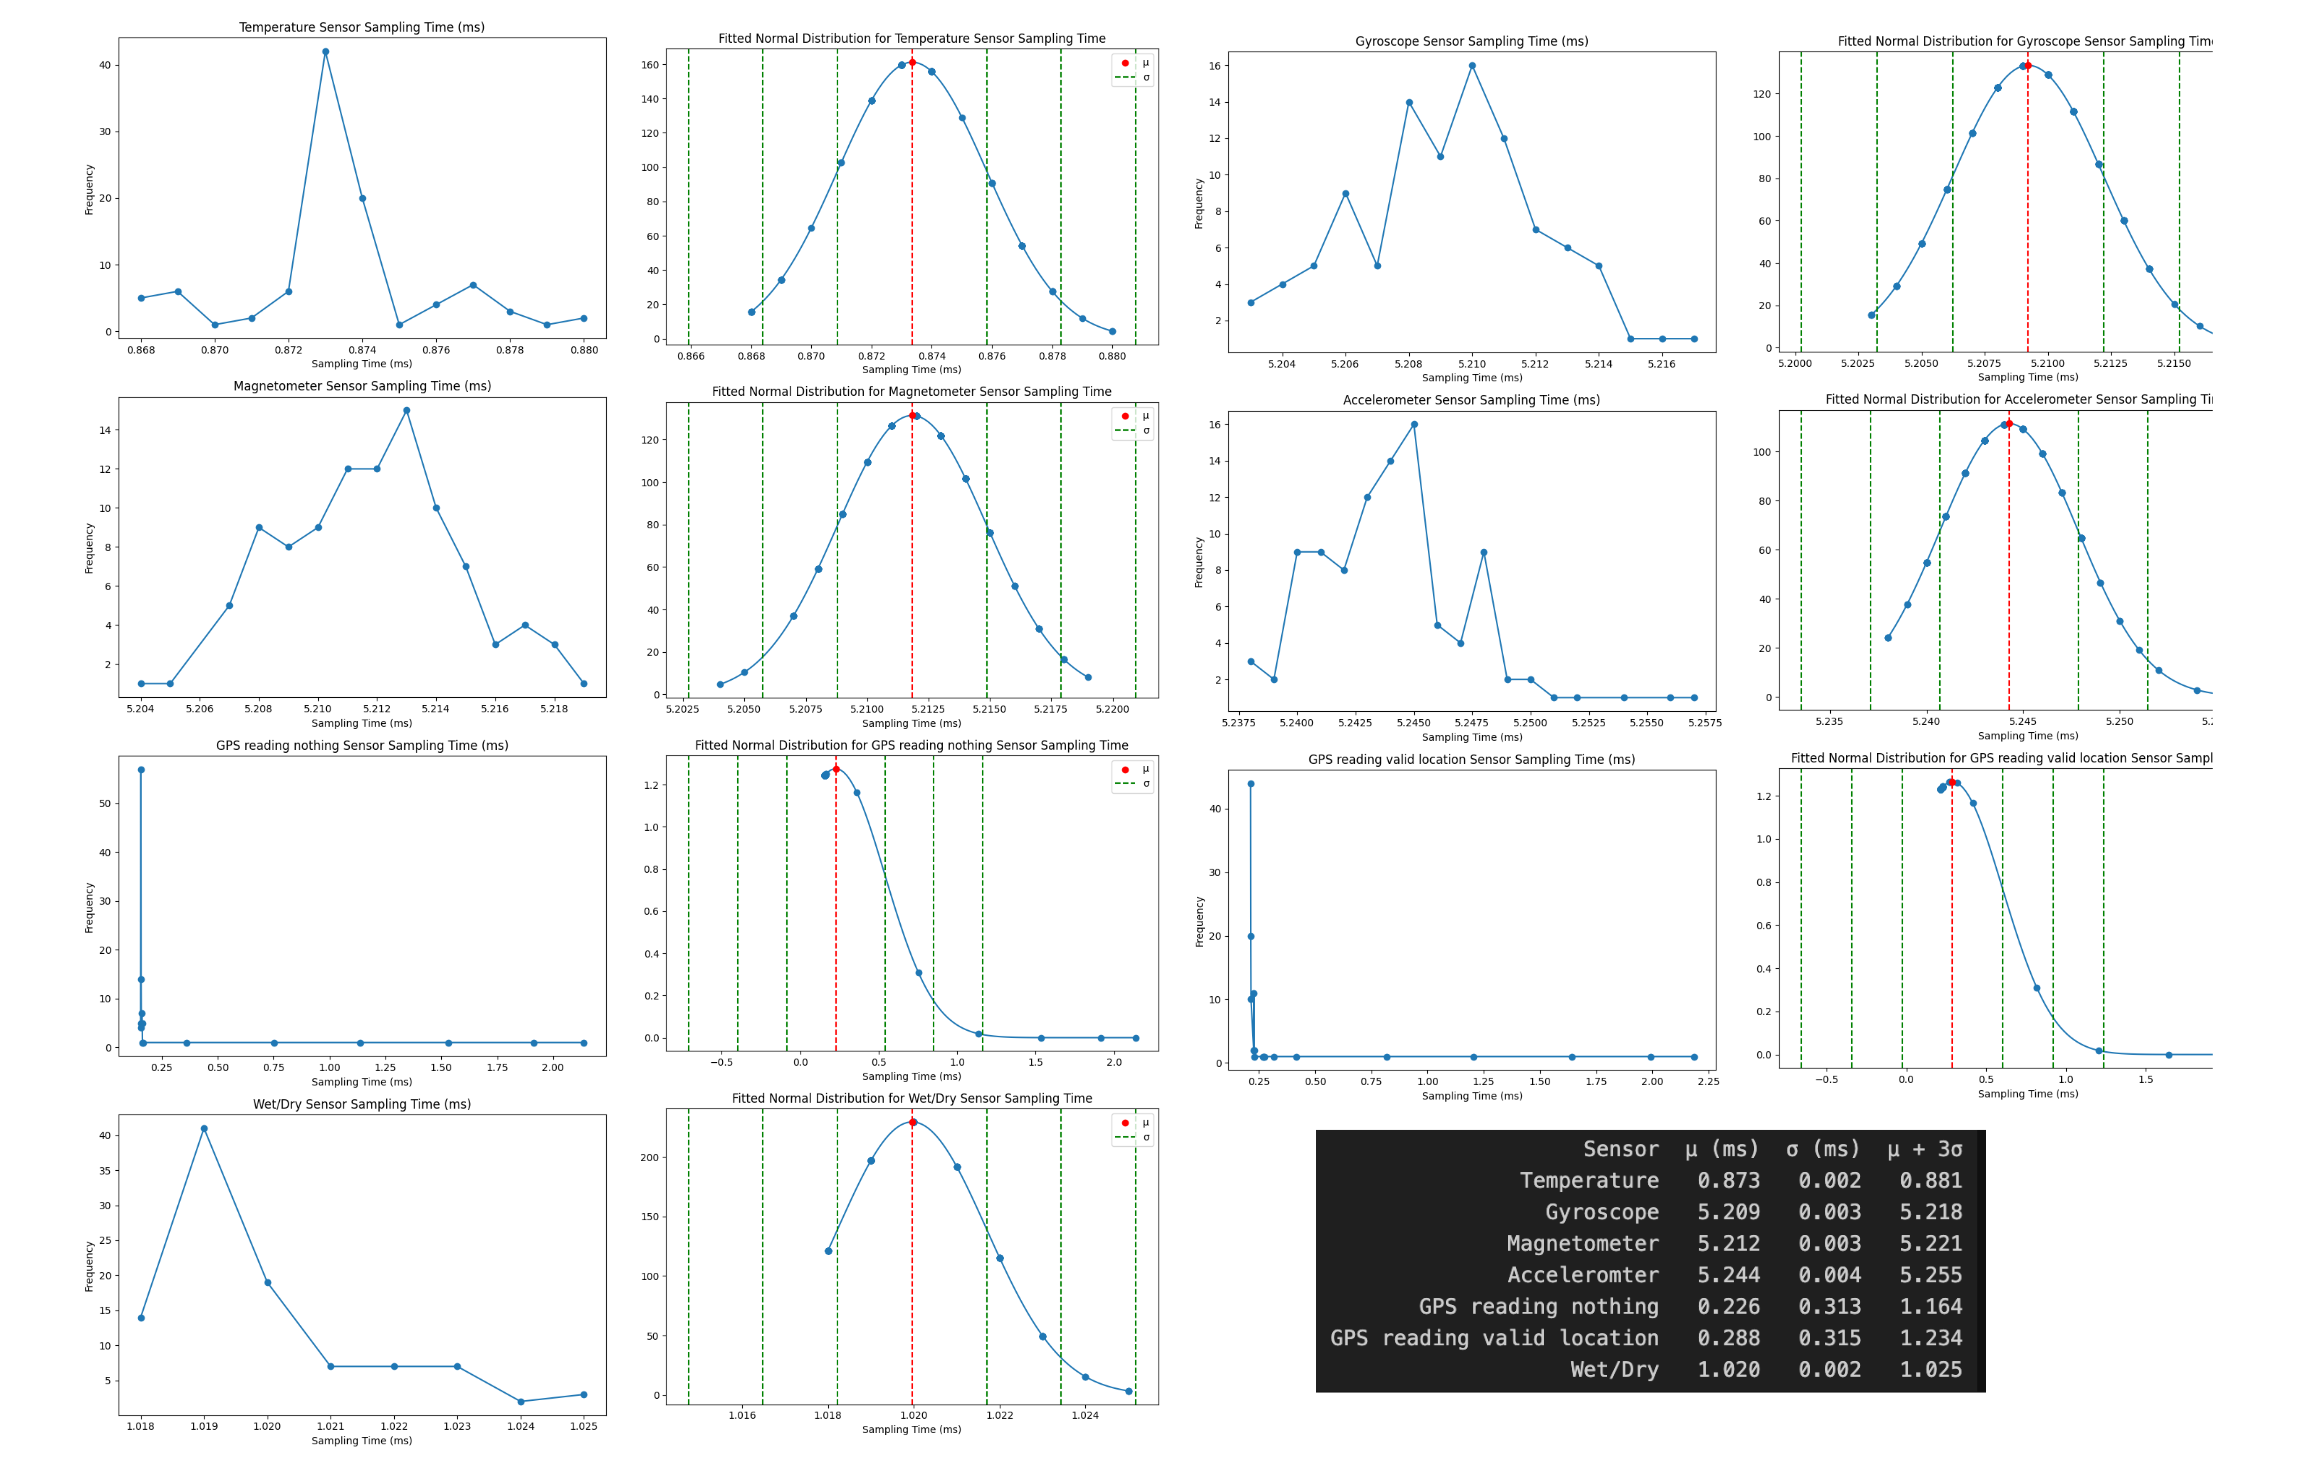
\includegraphics[height=0.8\textheight,width=0.8\textwidth,keepaspectratio]{images/samplingtimegraphs.png}
\end{frame}

\begin{frame}{Sensor Sampling Time Data}
    \centering
    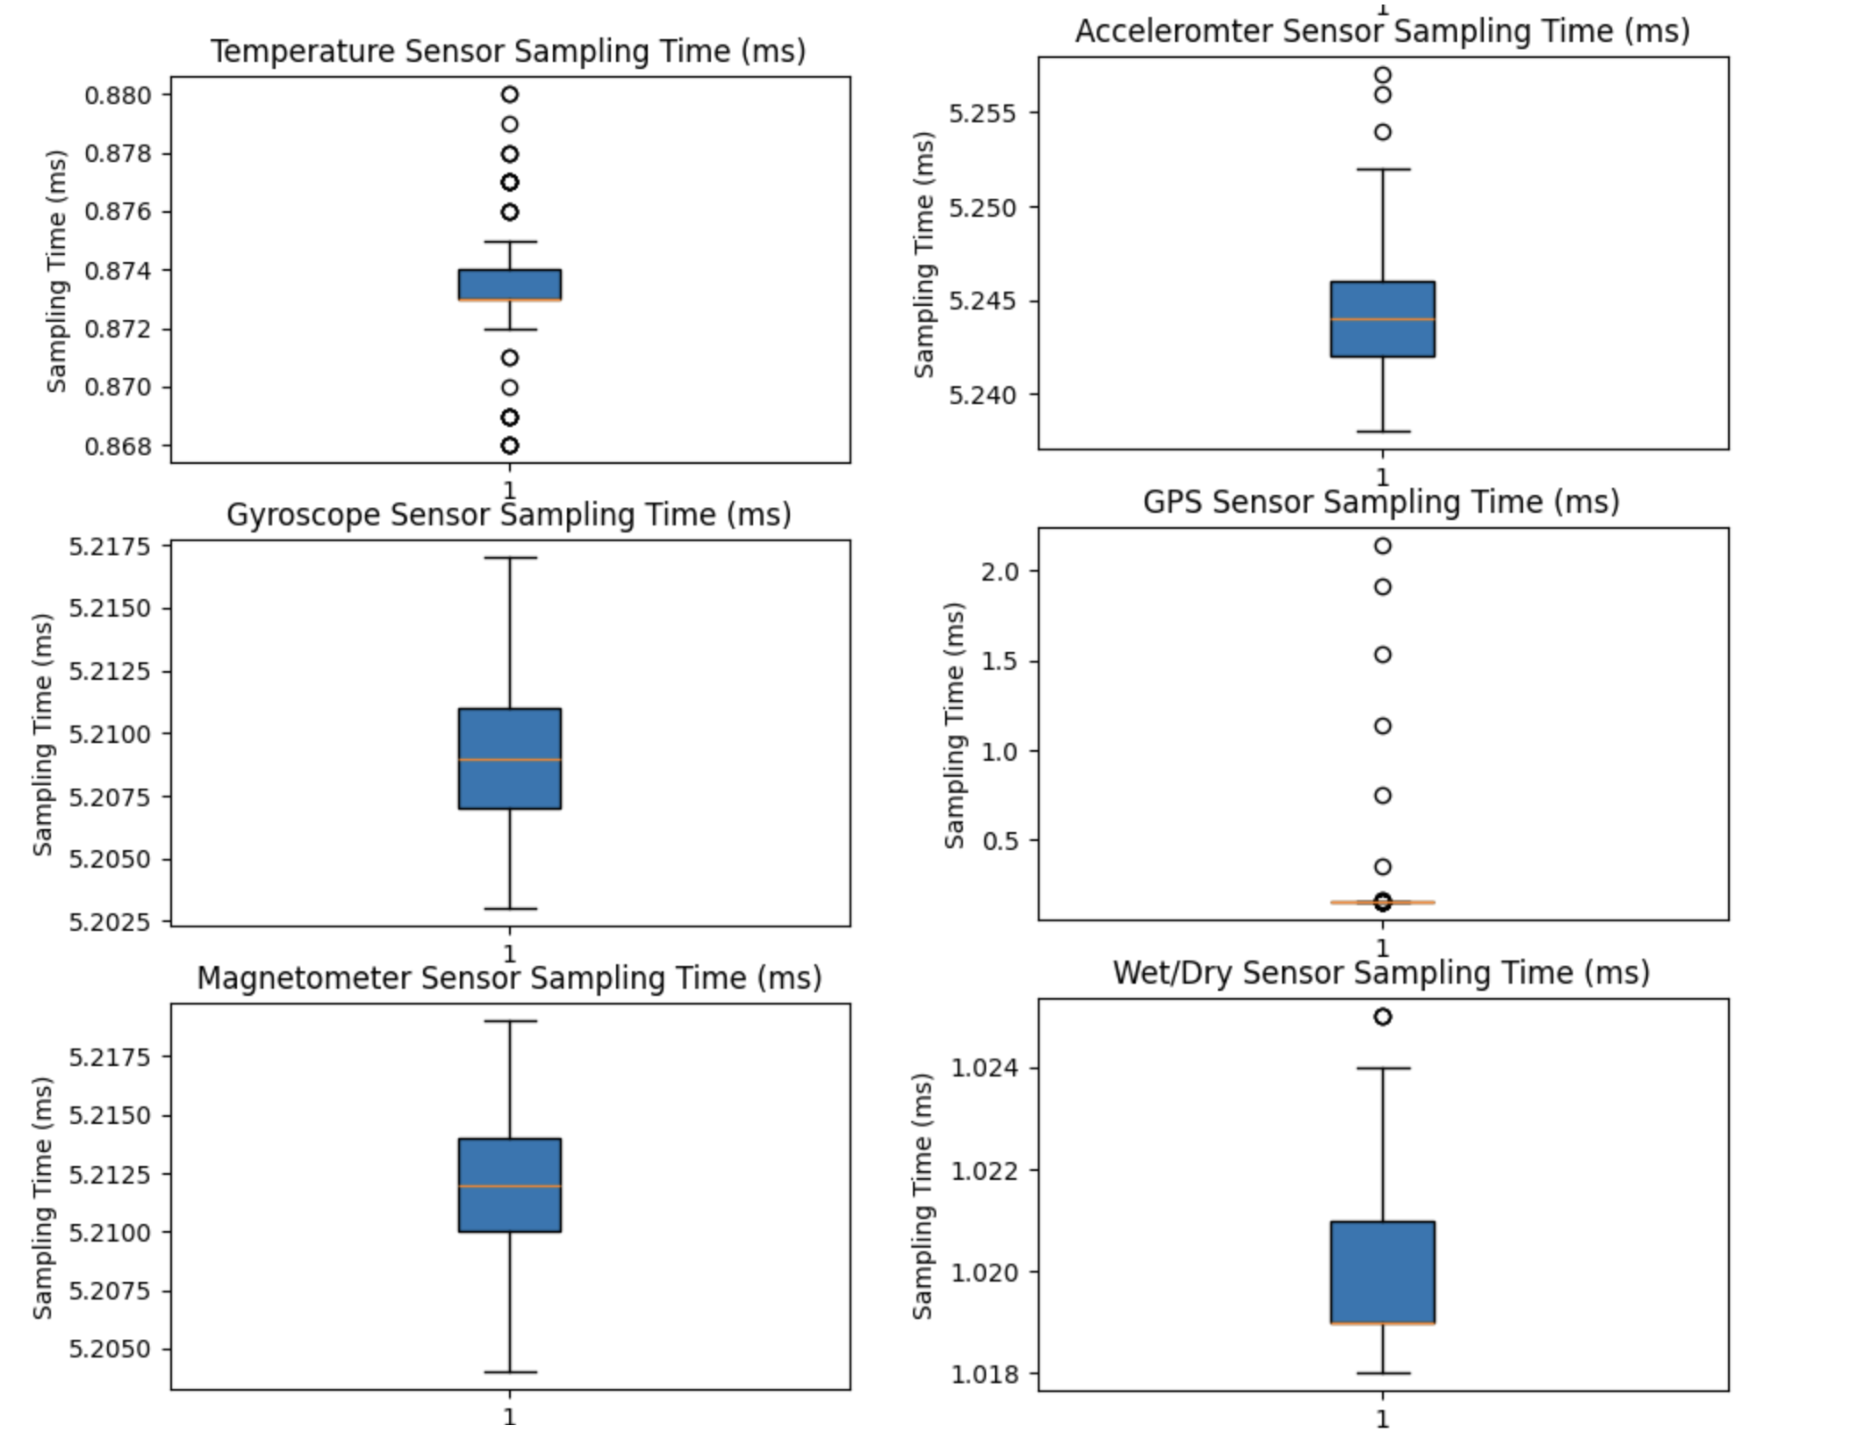
\includegraphics[height=0.8\textheight,width=0.8\textwidth,keepaspectratio]{images/boxplots.png}
\end{frame}

\begin{frame}{GPS Data}
    \centering
    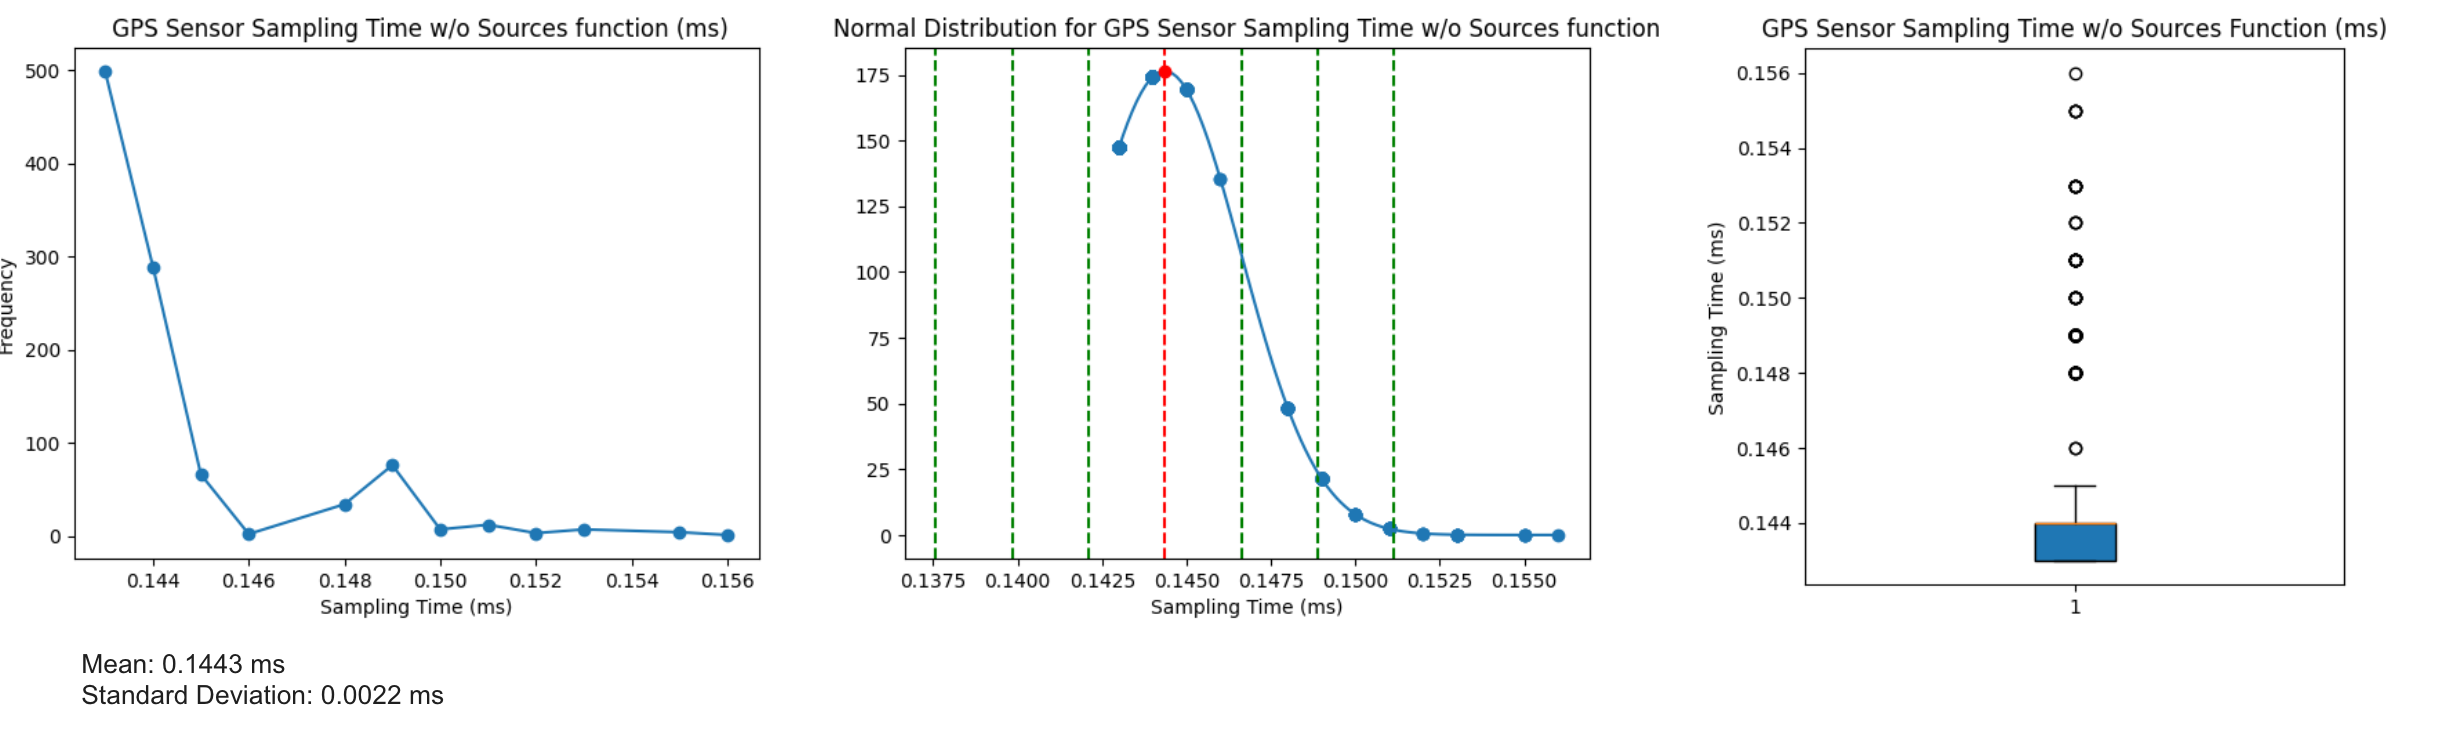
\includegraphics[height=0.9\textheight,width=0.9\textwidth,keepaspectratio]{images/gpsdata.png}
\end{frame}



\begin{frame}{Fourier Transform and Spectral Artifacting}
    \begin{columns}
        \begin{column}{0.5\textwidth}
            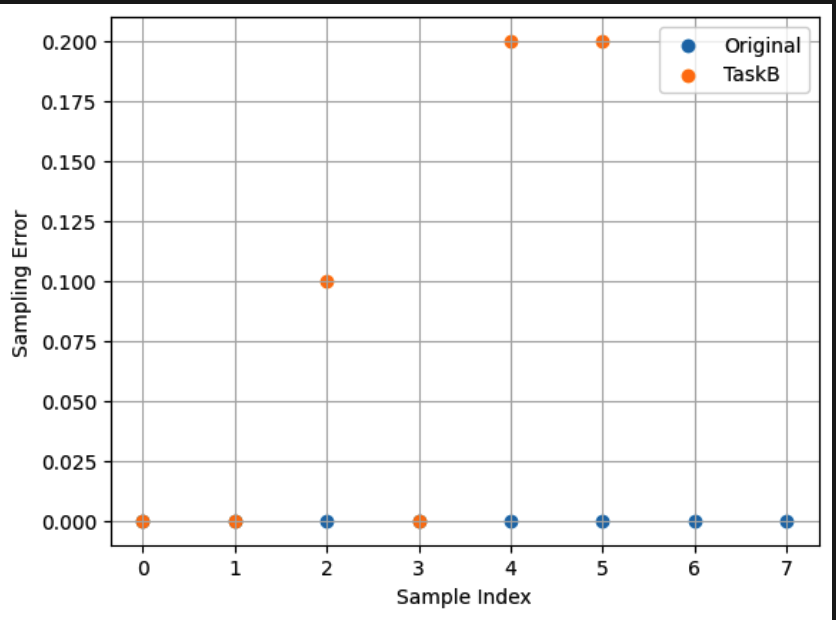
\includegraphics[height=1\textheight,width=1\textwidth,keepaspectratio]{images/Sampling_Error.png}
        \end{column}
        \begin{column}{0.5\textwidth}
            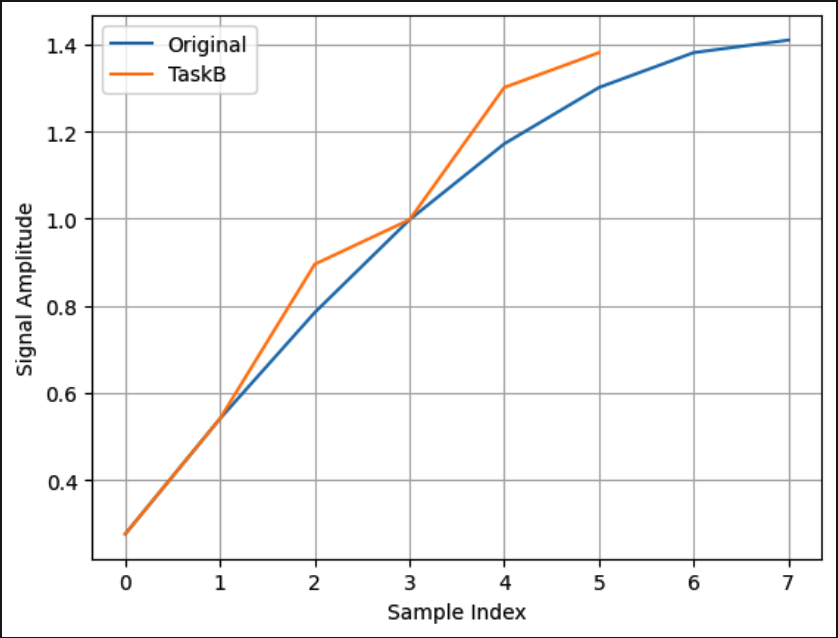
\includegraphics[height=1\textheight,width=1\textwidth,keepaspectratio]{images/Signal_Diff.png}
        \end{column}
    \end{columns}
\end{frame}

\begin{frame}{Fourier Transform and Spectral Artifacting}
    \centering
    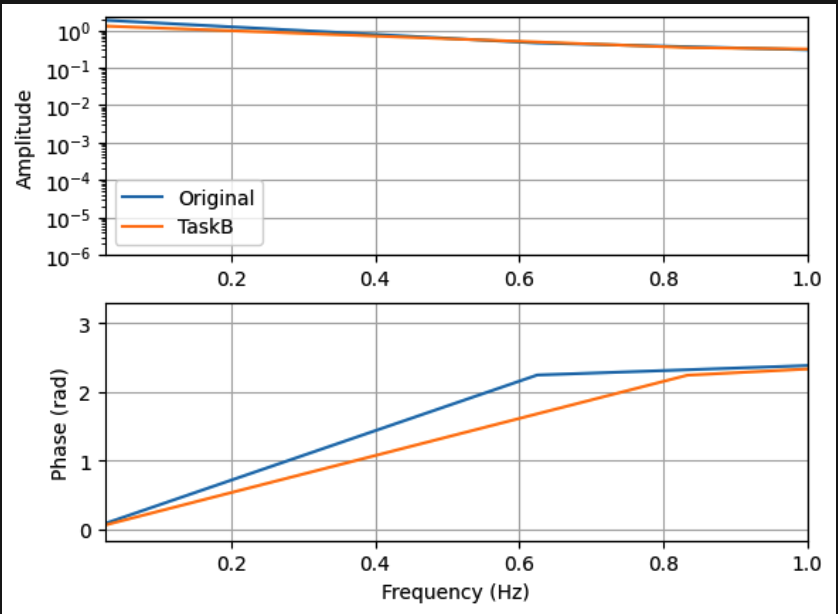
\includegraphics[height=0.8\textheight,width=0.8\textwidth,keepaspectratio]{images/Amp_Vs_Freq.png}
\end{frame}

\begin{frame}{Scheduler}
    \begin{itemize}
        \item Goal: Preserve intervals of each task as much as possible, with tasks ranked in priority
        \item Each task has an interval (time between runs), duration of task, and next run time 
    \end{itemize} 
    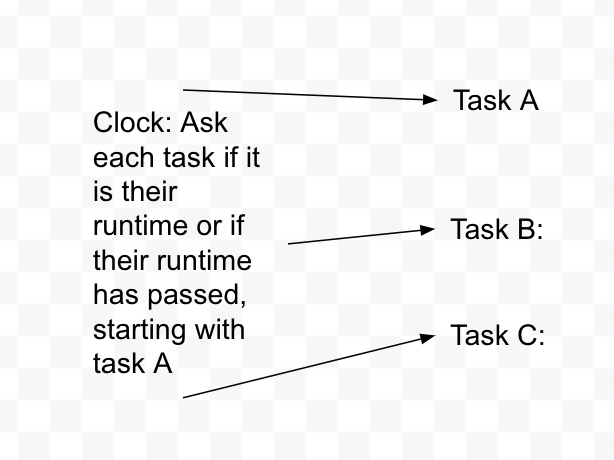
\includegraphics[height=0.5\textheight,width=0.5\textwidth,keepaspectratio]{images/schedulerPart1.png}
   
\end{frame}

\begin{frame}{Scheduler}
    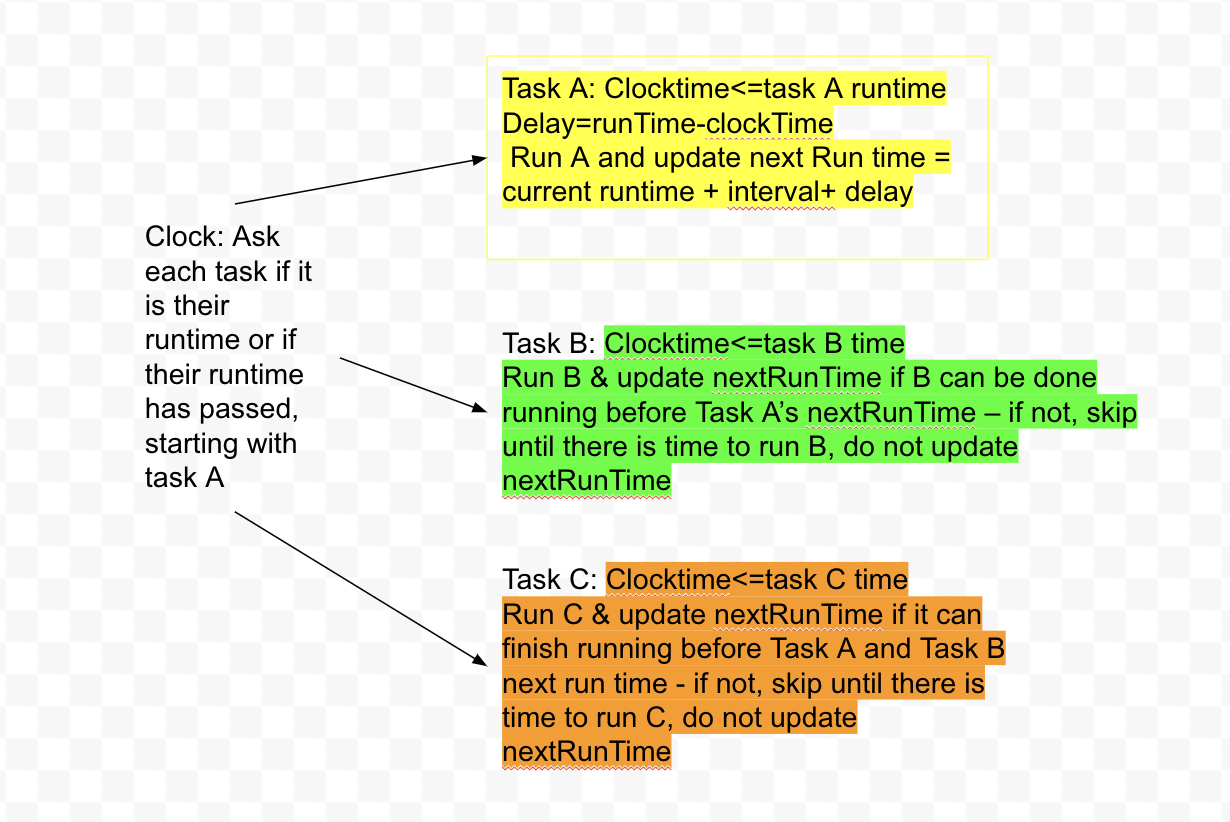
\includegraphics[height=0.8\textheight,width=0.8\textwidth,keepaspectratio]{images/schedulerPart2.png}
   
\end{frame}

\begin{frame}{Scheduler}
    \begin{itemize}
        \item Delay: If a delay is present, flag what tasks and when the delay occurred. Need for spectral analysis.
    \end{itemize}
\end{frame}



% To create a slide with two columns, use the following:
% \begin{frame}{TITLE}
%     \begin{columns}
%         \begin{column}{0.5\textwidth}
%             COLUMN 1 BODY
%         \end{column}
%         \begin{column}{0.5\textwidth}
%             COLUMN 2 BODY
%         \end{column}
%     \end{columns}
% \end{frame}
